
\documentclass{article}

\usepackage[utf8x]{inputenc}
\usepackage{graphicx}
%\usepackage{wrapfig}
\usepackage{verbatim}
%\usepackage{float}
\usepackage{caption}
\usepackage{subcaption}
\usepackage{hyperref} %NOTE: Must be the last 'usepackage'.

\begin{document}

\title{Poxelcoll version 0.1 manual}
\date{May 2012}
\author{Jens W.-Møller}
\maketitle

\tableofcontents

\listoffigures


\section{Intro}

Poxelcoll (\textbf{Po}lygon/pi\textbf{xel}-perfect \textbf{coll}ision detection library)
is a FOSS library designed to support easy, flexible and efficient pixel-perfect collision detection,
including simple transformations such as scaling and rotation.

\subsection{Overview}

This introduction starts with a background that describes the main motivation behind
the library, as well as the main idea of the library. It continues with
simple instructions for basic usage of the library, some general information
and issues regarding collision detection and this library, a part about
geometric and numerical stability, a discussion
of when this library may be useful or not (including potential substitutes).
It ends with a brief discussion of portability, license, status and future
of the library.

\subsection{Background}

2D game development frequently features some sort of physical world where
things can collide. The complexity of modelling and the used solutions
varies greatly, from simple grid-based models, to complex models
with accurate simulation of gravity, friction, momentum, etc.
The part of the modelling that deals with detecting collisions is commonly called
collision detection.
A major challenge for implementing solutions to the more complex models
is \emph{ease of use}, \emph{flexibility} as well as \emph{efficiency}.
The major factor that determines these issues is the basic representations
of collision objects, also known as primitives.
Simpler primitives tend to be more efficient
and easier and not very flexible, while more complex primitives are
much more flexible, but generally not very efficient, easy to use or implement.

For ease of use and efficiency, simple solutions include using
axis-aligned bounding boxes or perfect circles. While these solutions
are very simple, they are not flexible at all, and may limit the gameplay
of the games that use them, solely due to technical limitations.

Another solution which is much more flexible is that of pixel-perfect collision detection.
Pixel-perfect collision detection uses images as a spatial representation of the
collision object. This is conceptually easy, especially if the image used for
the primitive is the same as that which is used for drawing: if a sprite is
seen to collide on screen, it also collides in the game.
Since most 2D games, libraries, tools and engines has some
support for images and sprites, handling images is generally not an issue.
If basic transformations such as scaling and rotation is supported dynamically,
it is also very flexible. Examples of games that uses pixel-perfect collision
detection include the 2D games of the Worm series.

The main issue with pixel-perfect collision detection is that it is difficult to
implement efficiently, especially if basic transformations is supported dynamically.
Simple implementations, without any transformation, goes through each pixel of one
image and checks if it is filled at the same time as the corresponding pixel
in the other image is filled. Even if optimised, this is generally very inefficient.
The problem becomes worse when the images needs to be transformed,
because every time the transformation changes for a given collision object,
the whole image, along with every pixel in it, needs to be changed.
If pixel-perfect collision detection is used or needed for the gameplay,
it can limit the game to small and few collision objects.

A third, general solution is to use complicated or multiple geometric primitives
to represent the collision objects. For instance, convex or concave polygons,
using multiple triangles, boxes, circles, lines, etc. can be used here.
When the desired collision shapes fits well with the geometric primitives,
it can be very efficient.
There are many options, and it can be somewhat flexible, especially if many
primitives is used for each collision object. Transformation is also somewhat
efficient, since geometric primitives are described by relatively few points.

However, it is not always easy to use. If the desired collision shape does not
fit well with geometric primitives, approximating it may take time
and energy, may not be efficient (due to the number of primitives used),
and may not be as precise as desired.

The \textbf{main idea of this library} is to combine the pixel-perfect collision detection
with a general geometric primitive, namely the convex polygon.
The convex hull of the collision object's image is precomputed and stored.
Whenever the collision object must detect collisions with another collision object,
the convex hull is transformed with the basic transformations (rotation, scaling).
Since the convex hull consists of comparatively few points, this will generally
be efficient. The same is done for the other collision object.
With the two transformed convex hulls, a precise intersection between them is found.
This intersection is the only part which needs to be checked for collisions using
the backing images, since the images will definitely not overlap outside
the intersection.
Another advantage is that this enables easy and efficient collision detection
between pixel-perfect collision objects and geometric collision objects.

\subsection{Getting started}

First, pick between the Scala and C++ implementation.
The Scala implementation is (of version 0.1) faster and
has slightly more features, and should be preferred when the JVM
platform is used. The C++ implementation is preferrable when
the platform is not JVM, simply because Scala (as of this writing)
essentially requires the JVM.

Next, read the installation for the given implementation
in the document "INSTALL".

Once the library has been setup and is ready to use,
look at the API documentation for the BinaryImage,
Mask and CollisionInfo classes, in that order.
These are some of the main data types when using the library.
The BinaryImage represents an image, where each pixel
is either on or off. The images that is to be used for
collision detection should be loaded into BinaryImage's.
The mask represent a collision primitive.
It consists of an optional BinaryImage, an origin
around which transformations happen,
a bounding box which covers the whole image,
as well as a convex hull.
For ease of use, factory methods are provided
that automatically generates both the bounding
box and the convex hull given a binary image
and origin point.
The final class is CollisionInfo, which
holds a Mask, some collision information
such as rotation angle and scaling along
x-axis and y-axis, and an id.
While the Mask is meant to be permanent and precomputed,
the CollisionInfo is more temporary.
The id indicates which object the collision object
belongs to.

If images are not always used, the ConvexCCWPolygon must be
understood and used when creating the mask.
Be careful about obeying its contract! Without obeying
its contract, the library gives no guarantees in regards
to correctness or efficiency.

Those classes are the main things you have to worry about.
Once you have those set up, simply use the Pairwise
class to detect collisions. However, it is recommended
that you read or at least skim through the rest of the
manual to understand what is going on, and to know
about the issues in the library.

\subsection{When this library is appropriate}

This library is not suitable for 3D collision detection,
nor is it suitable for platforms where Scala or C++ is not
supported or appropriate.

Furthermore, its license is GPLv3, which may cause problems for some potential users
of this library.

If the issues regarding numerical stability matters, this library is not appropriate at all.
Look into libraries like CGAL.

If pixel-perfect collision detection is not used or needed, there may exist libraries
out there which are more suited to the given context. However, if convex hulls
represented by convex polygons are efficient, flexible and easy enough for the required
purposes, this library may suit the purposes.

If a fully-fledged physics engine is required, this library alone is not enough.
The library has not been built to support or to be incorporated into a physics engine,
and while it may or may not be possible with few modifications, it has not been investigated.
However, if a physics engine with pixel-perfect collision detection is desired or needed,
incorporating this library into an existing physics engine may be the best solution.
For physics engines, box2d is a 2D physics engine written in C++ with a permissive license.

For contexts where the images change, for instance for games where destructable terrain
is featured, the efficiency of this library may or may not be sufficient. The library
requires precomputation of the images for finding the convex hull. This presents two
issues. The first is that the repeated recomputation of the convex hull may be too inefficient.
This depends partly on how frequently images change in the worst case.
The second issue is that images that fitted the convex hull well before the change
does not fit the convex hull well after the change. The effect on performance can be considerable.
Prototyping the library and seeing if its performance is acceptable may be the best option,
but it is in any case recommended that the different aspects that affect performance of the library
is understood clearly before taking any decisions.

For pixel-perfect collision detection systems where basic transformations like rotation and scaling
is not required, it depends on the context whether this library should be used, but for most
contexts this library should perform efficiently. Even if the basic transformations are not used,
this library may be several orders of magnitude more efficient than the naive alternatives
in the best case, and only a low constant-factor slower in the worst case.
See the section regarding efficiency for more information.

Overall, if you need pixel-perfect collision detection, this library (either pure, modified or
combined with another existing library) should be suitable for your purposes.

\subsection{Portability}

NOTE: This pertains to version 0.1.

The portability depends on the implementation used.

For the Scala implementation, there is no dependencies on other libraries,
and the implementation can thus be used on any platform that supports Scala.
The language version used is 2.9.2.
The only external dependencies that may be introduced is that of Swing,
and then only for parts unrelated to the library itself, such as
testing, performance profiling and demonstration.
sbt is used for compiling and generating documentation.

For the C++ implementation, C++11 is used extensively in the implementation.
Therefore, only platforms with compilers that support C++11 can be used.
There are also a few dependencies on Boost, notably dynamic\_bitset
and array.
The make system also happens to be hard-wired to use g++ with compiler
flags for using C++11. Changing the make system for someone experienced
with system administration should in theory be easy, and help would be
appreciated. CMake is used to generate makefiles, and doxygen is used for
generating documentation.

\subsection{License}

The entire library is licensed under GPL v3. For more details, see the document
"LICENSING".

The main reason is that it encourages users to share and improve the library.
By ensuring that everyone who uses the library keeps it open source,
everyone can modify and change it, and improvements from all users can be
redirected to the library, improving the library for all.
Furthermore, it means that the real-world usage of the library can be investigated,
and the library can then be changed and improving based on actual usage and needs.
It also guarantees the freedom of users to use the library as they want to.

Another reason is that a fair amount of work was put into this library,
and it is released in the hope of contributing to the game development
community as well as the FOSS community. Without a proper license,
proprietary users could use this library gratis and without any effort,
thus not contributing anything back.

If you want to use this library in a project, ensure that it is compatible
with the GPL v3.

\subsection{Status and future of the library}

As of version 0.1, 2012-05-08, the \textbf{status} is that the library is somewhat stable and well-documented.
It does not have many features, but does have the most important ones
(efficient pixel-perfect collision detection, efficient basic transformations).
The library has never been used in the real-world, and there are no regression
tests.

The Scala version is more mature than the C++ version.
The reason is that the C++ version is basically a nearly-direct translation
of the Scala source, which means that it is not idiomatic C++, and that
it seems to be a lot slower than the Scala version in basic performance tests.

For the \textbf{future}, three areas can be improved upon.
In the following, they will be described in decreasing priority,
starting with the highest priority.

The first area is stability, correctness and testing of the library.
The reason this is the highest priority is that making the library
correct is non-trivial, and if the library is not correct and robust,
it is not very useful. Issues like geometric stability
and numerical stability makes this area harder to maintain and improve.
More regression tests, demonstrations and performance tests will
make the library more reliable. Real-world usage may also uncover
other issues. In regards to known issues, the best improvement would
be ensuring numerical stability, or at least determine what effects
numerical instability has on the current implementations.

The second area is more features. One possible option is support for
broad phases. This is not a big necessity, since other libraries
already provides this functionality, and pixel-perfect collision
detection does not have different requirements than other collision
detection systems in regards to the broad phase.
Another option is support for only colliding with pixel of a
certain transparency, getting the collision point, etc.
These are smaller features that would take some work,
and if someone needs them, it should be entirely possible
to fork/modify the library to handle them.
Another area is improved precomputation. While the pixel-perfect
collision is generally efficient for images that are accurately approximated
by their convex hull, they are not necessarily efficient for images
that are not approximated well by their conevx hull.
One possible option to handle this is to split the image into smaller
parts, and find the convex hull of these smaller parts.
If the number of parts is small, and these parts are generally
well approximated by their convex hull, this may increase the
efficiency. Providing a general algorithm that automatically
determines if and how to split an image might improve the
efficiency and the ease of use of the library.
Other features would include changing and expanding the
API such that it fits better with real-world usage.

The third area is efficiency, both asymptotic and constant-factor. While the library should be
reasonably efficient, there are room for improvements in many
places. However, flexibility, maintenance, robustness and correctness is more
important, and this area can always be improved upon incrementally
as performance profiling indicates which parts it is worth
making more performant.




\section{General topics}

This part introduces general background topics, and how they
pertain to the library.

\subsection{Collision detection}

Collision detection deals with detecting collisions between
collision objects. In many cases, collision detection is a
challenging area, primarily because it is difficult to both
make solutions flexible, easy to use and efficient.
Especially efficiency is very often a large issue.
Since different domains have different requirements in regards
to flexibility, ease of use and efficiency, different solutions
are appropriate in different cases. Nonetheless, there are
some parts of the handling that are general to how the problems
can be approached.

In many domains, the issue of efficiency stems not only from the
complexity and accuracy of the individual collision objects,
but from the possibly large number of different collision objects that may
collide. Since collision objects frequently model spatial objects,
and thus rarely overlap or are all placed on top of each other,
most collision objects are far away from each other.
In some cases, even checking for all objects which objects they
are far away from is too inefficient. For instance, checking
for each of 10.000 objects which of the other objects they are
far away from requires in the brute-force implementation 100.000.000 comparisons.
Depending on the specific context, there exists different
solutions and ways to handle this problem,
having much fewer comparisons than in the naive implementation.
This phase of collision detection is commonly called the broad
phase.

In contrast, the narrow phase of collision detection only deals
with pairs of objects. For complicated objects that are expensive
to detect collisions for, there exists methods such as bounding
volumes to handle it. A bounding volume is one or more over-approximations
of the actual object that are more efficient to check for than the
object itself. The advantage is that if there is no collision,
the checking of the bounding volumes may determine that there is
no collision, and thus the more expensive collision detection is avoided.
Variations on this includes bounding volume hierarchies.
In this library, the over-approximating bounding volumes is primarily
the axis-aligned bounding box and the convex polygon for the convex hull.
The axis-aligned bounding box is less precise but faster, while the
reverse is true for the convex hull.

This library deals exclusively with the narrow phase as of version 0.1.
If the broad phase of the collision detection is not efficient enough,
this library can be combined with other libraries or solutions
that handles it better.

\subsection{Geometric and numerical stability}

Geometric stability and numerical stability are two important properties
in computational geometry. Since this library contains elements of
computational geometry, it is important to discuss these properties
in regards to the library.

Geometric stability is about considering and handling all geometric cases correctly
in a computational geometry algorithm, no matter what kind of input is given.
As an example, an algorithm that finds the intersection between two convex polygons
that finds the correct answer most of the time, for instance when the intersection
is a polygon itself, but fails in some way (crash, wrong answer, infinite loop, etc.)
for the cases where the intersection is a line, a point or is empty is not geometrically
stable. Conversely, an algorithm that always finds the correct answer no matter what the
intersection is, is geometrically stable.
All algorithms in the library are designed to be geometrically stable, and seems to
be geometrically stable in tests.

Geometrical algorithms frequently assumes that calculation with numbers has infinite
precision. This is not true in general. When an algorithm that would be correct
if the precision was indeed infinite, but is wrong when it isn't, it is because the
algorithm is not numerically stable. This is a big problem in computational geometry
because even small errors can have large consequences. While in other fields finite
precision for numbers mostly means decreased precision, it can in computational
geometry lead to errors, wrong answers, crashes, infinite loops, etc.
An example is testing the cross product of two vectors.
If a rounding error gives a wrong result (ie. negative result instead of positive),
a different decision branch of the algorithm may be taken.
The consequences and effects of numerical stability are fully unknown as of version 0.1,
and even though they have not caused problems in tests so far, it does not mean
that they cannot produce undefined behaviour given certain input.
For this reason, this library should not be used for scientific or mission-critical
purposes, nor for any purposes where the potential consequences of numerical stability
are not acceptable. This issue may or may not be improved upon in the future.



\section{Documentation}

This section contains the general documentation of the library,
explaining the data types and important features,
as well as how and why certain parts are implemented the way
they are. It also describes details related to efficiency,
as well as the Scala and C++ implementations.


\subsection{General data types}

The library provides a number of general data types.
By "data type" is meant basic data containers that
represent different concepts and support different
operations. For instance, a mathematical vector contains a couple
of coordinates, and supports operations like cross-product
and dot-product. Having a precise understanding of the data types
in the library makes it easier to use the libray.

A general note about the data types in the library is that they
are, in general, immutable. This makes it generally easier
to reason about the library and ensure that it is robust
and correct.

The most important of the data structures in regards to using
the library is the BinaryImage, Mask and CollisionInfo.
If polygons are used as primitives, it will be necessary to use
ConvexCCWPolygon as well.

\textbf{BinaryImage} represents an image. By an 'image' is meant
a 2-dimensional finite area of values, that have a width and a height.
A 'binary image' is an image that holds binary values, meaning that
each value in the image is either 'on' or 'off', or alternatively,
1 or 0. In the library, binary images are used as the primitive for
pixel-perfect collision detection. 'on' or 1 represents that there
is something, while 'off' or 0 represents that there is nothing.
When the binary images of two collision objects overlap,
and there is at least one point in the overlap where both of the
binary images is 'on' or 1, there is a collision. If not, there
is no collision.

The way to construct a pixel-perfect binary image from an image
depends on the image, but usually the transparent/background pixels
are mapped to 'off', while the foreground/not transparent pixels are mapped
to 'on'. Done this way, if the image collides visually with something,
it collides with that same thing in the collision system.

There is a basic abstraction for factories for binary images,
which takes a sequence of rows of 'on'/'off' values, ie. boolean values.

\textbf{Mask} is the main abstraction for collision primitives.
It consists of a origin, an axis-aligned bounding box,
a nonempty convex hull, and an optional binary image
(for more information on what a convex hull is, see wikipedia).

As of version 0.1, it has two potential meanings:
If it has a binary image, it is a pixel-perfect primitive
using the binary image for the pixel-perfect part and
using the axis-aligned bounding box and the convex hull
for bounding volume collision pruning
(for example, if the bounding boxes of two collision primitives does not
overlap, the more expensive collision checking is skipped).
In that case,
both the axis-aligned bounding box and the convex hull
should be precise or over-approximating,
and never under-approximating the binary image.

If instead it does not have a binary image,
it means that it is a polygon-based primitive
using the convex hull for the polygon
and using the axis-aligned bounding box for
bounding volume collision pruning.
The bounding box should be precise or over-approximating
the convex hull, and never under-approximating the
convex hull.

The origin point indicates for the three other parts
(the optional binary image, the convex hull,
and the axis-aligned bounding box).
So, if a point in the mask has position (1, 2),
and the origin point is (5, 5), the effective
position of the point in the mask is (-4, -3).
Setting the origin point the right place is important.
It is the point about which rotations happen, and if
a collision mask is placed at global position (0, 0),
then the point in the mask that correspons to the
origin will be found at global position (0, 0).
For more information regarding coordinates and points,
see P.

Finally, it should be noted that Mask is meant
to be precomputed in some ways. Some parts of it,
such as the convex hull, can take O(n log n) time
to compute,
where n is the number of pixels in the binary image.

\textbf{CollisionInfo} represents a collision object
in a specific state.
It contains a collision primitive,
a position, an angle for rotation, a scaling factor
in the x-axis and the y-axis, and finally the id
of the collision object.

The order of transformation for finding the final positions
of the collision primitives pixels is: origin, scaling, rotation, position.
First the pixels are translated according to the origin,
then they are scaled along the x-axis and the y-axis.
Then they are rotated by the angle, and finally
translated by the position.

For no transformations, the scaling factors should both be
1.0, and the rotation should be 0.0. The translation
vector should be (0.0, 0.0).

The angle is measured in radians, the position in pixels,
and the factors are percentages - so 1.0 is no scaling,
2.0 is double as big along the axis, and 0.5
is half as big along the axis.

\textbf{P} represents a simple 2D-point,
with an x-coordinate and a y-coordinate.
The x-coordinate goes along the 1. or horizontal
axis, and the y-coordinate goes along the 2. or
vertical axis. The units are generally pixels.

In some places of the API, a simple 2D-point
is viewed instead as a 2D-vector. For that reason,
P supports several operations for vectors,
such as cross-product and dot-product.

\textbf{IP} is simply a less feature-full
integer-version of P.

\textbf{BoundingBox} is an axis-aligned bounding box.
It consists of two points, of which the minimum
represents the corner of the axis-aligned box
that is the closest to origo, and the maximum
represents the corner of the axis-aligned box
that is the furthest away from the origo.

BoundingBox supports efficient intersection
checking. It is used as the most inaccurate
bounding volume: it generally over-approximates
a lot, but is very quick, making it useful for
pruning collision objects that are far away from
each other quickly.

\textbf{CollisionPair} is a simple representation
for two collision objects that collide. Since a
collision object cannot collide with itself,
the ids for a CollisionPair may never be the same.
For consistency and comparison, the first id
must always be strictly smaller than the second id.

\textbf{ConvexCCWPolygon} is the superclass for representing
convex polygons. Convex polygons are especially suited for
representing convex hulls. ConvexCCWPolygon has 4 concrete
subclasses, which are disjoint and which together represents
all legal ConvexCCWPolygon's: Empty, Point, List, and Polygon.

\textit{Empty} is the convex polygon that represents no points.
It is mainly included to ensure that all cases are considered
through the type system.

\textit{Point} is the convex polygon that represents exactly one point.

\textit{Line} is the convex polygon that represents a line segment,
described by two points, both of which are included in the line segment.
The points may NOT be the same. For the case where they are the same,
Point must be used.

\textit{Polygon} is the convex polygon that represents a polygon with
non-zero area. Thus, it has at least 3 points, none of which are collinear.
There is a number of important restrictions on Polygon. The first is that
it has 3 or more points. The second is that none of the points are equal.
The third is that the polygon they represent is 'simple'
(see http://en.wikipedia.org/wiki/Simple\_polygon for more information).
The fourth is that the polygon they represent is convex.
The fifth is that the polygon is defined counter-clockwise, such that
if the first three points are named p1, p2 and p3 in that order,
and v1 is the vector |P1 P2|, and v2 is the vector |P2 P3|,
then the cross product of v1 and v2 will be strictly positive.
The sixth is that none of the points are collinear.
The seventh is that the area of the polygon is non-zero.
If these restrictions are not obeyed, the library's efficiency,
accuracy or correctness cannot be guaranteed.
One simple way to construct a correct convex polygon is simply to
make a couple of points where the corners of the polygon should be,
and then use the convex hull algorithm defined in the library
under the name ConvexHull to get the corresponding correct polygon.
The ConvexHull algorithm is robust, and will always give a valid result
no matter the input.

In some cases, a subset of the different polygon cases are needed.
Examples of this includes the \textit{NonemptyConvexCCWPolygon},
\textit{EmptyPoint} and \textit{EmptyPointLine}.
The first includes all concrete types except Empty,
the second includes only Empty and Point, and the third includes
Empty, Point and Line.




\subsection{Basic transformations}

The basic transformations that are supported include
translation, rotation and scaling along the x-axis
and the y-axis. The order of transformation is
origin, scaling, rotation, translation.

Transformations are controlled through the CollisionInfo
data type.

It should be noted that some transformations make
collision objects uncollidable. These cases include
when either scaling factor is 0. In these cases,
the object causes no collision. The reason is that
such a scaling factor does not make a lot of sense,
because the object in question would have zero width/height.

As an example of basic transformations, consider a 4-by-4 rectangle
with an origo in the corner marked by the blue cross.
A transformation by translation P(0, 2), rotation 30 degrees
(in the library, it would be $\pi / 6$ radians), scale-x = 1.5
and scale-y = 0.5.

The initial mask is shown in figure \ref{fig:before_transformation},
while the result of the transformation is shown in figure \ref{fig:after_transformation}.

\begin{figure}[p]
	\centering
	\begin{subfigure}[b]{0.3\textwidth}
	  \centering
	  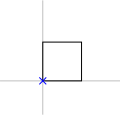
\includegraphics{transformations/before_transformation.pdf}
	  \subcaption{Before transformation}
	  \label{fig:before_transformation}
	\end{subfigure}
	\begin{subfigure}[b]{0.3\textwidth}
	  \centering
	  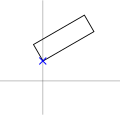
\includegraphics{transformations/after_transformation.pdf}
	  \subcaption{After transformation}
	  \label{fig:after_transformation}
	\end{subfigure}
\caption{Transformation, before and after}
\label{fig:transformation}
\end{figure}

In the implementation of the engine, transformations are done by
a 3-by-3 matrix, even though the coordinates are only 2-dimensional.
The reason is that working with a single matrix for transformations
and inverse transformations is simple and fast.
If only scaling and transformation was supported,
a 2-by-2 matrix would be sufficient. But since translation is
also supported, a 3-by-3 matrix is needed.
The reason is the same as to why 4-by-4 matrices are used in
3D graphics, even though only 3 dimensions are used.
See also \url{http://en.wikipedia.org/wiki/Homogeneous_coordinates#Use_in_computer_graphics}.




\subsection{Polygon intersection}

%TODO: What polygon intersection is.

Polygon intersection as understood in the library
is the intersection between two convex polygons.
It can be easily seen that the intersection between
two convex polygons is also a convex polygon.

The intersection is best illustrated through graphical examples.
The red polygon is the first convex polygon, the blue polygon
is the second convex polygon, and the violet area (if any) is the intersection:

\begin{figure}[p]
	\centering
	\begin{subfigure}[b]{0.3\linewidth}
	  \centering
	  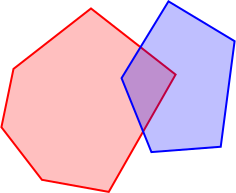
\includegraphics[scale=0.5]{intersections/intersection_simple.pdf}
	  \subcaption{Simple intersection}
	  \label{fig:intersection_simple}
	\end{subfigure}
	\begin{subfigure}[b]{0.4\linewidth}
	  \centering
	  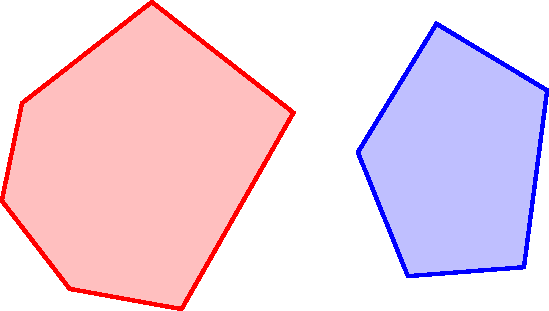
\includegraphics[scale=0.5]{intersections/intersection_none.pdf}
	  \subcaption{No intersection}
	  \label{fig:intersection_none}
	\end{subfigure}
	\begin{subfigure}[b]{0.3\linewidth}
	  \centering
	  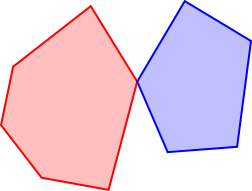
\includegraphics[scale=0.5]{intersections/intersection_point.pdf}
	  \subcaption{Point intersection}
	  \label{fig:intersection_point}
	\end{subfigure}
	\begin{subfigure}[b]{0.3\linewidth}
	  \centering
	  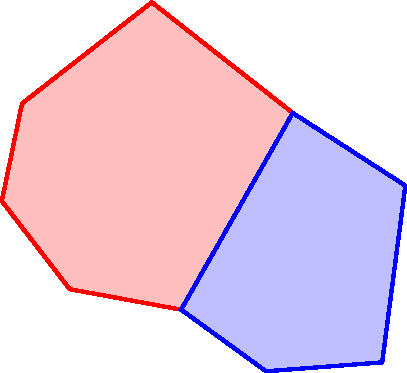
\includegraphics[scale=0.5]{intersections/intersection_line.pdf}
	  \subcaption{Line intersection}
	  \label{fig:intersection_line}
	\end{subfigure}
	\begin{subfigure}[b]{0.3\linewidth}
	  \centering
	  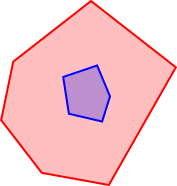
\includegraphics[scale=0.5]{intersections/intersection_inside.pdf}
	  \subcaption{Polygon inside intersection}
	  \label{fig:intersection_inside}
	\end{subfigure}
	\begin{subfigure}[b]{0.3\linewidth}
	  \centering
	  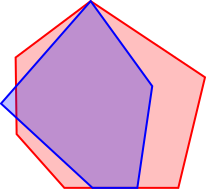
\includegraphics[scale=0.5]{intersections/intersection_fun.pdf}
	  \subcaption{Complex intersection}
	  \label{fig:intersection_fun}
	\end{subfigure}
\caption{Intersections}
\label{fig:intersections}
\end{figure}

As can be seen in figure \ref{fig:intersections}, convex polygon intersections can produce not only empty
and full convex polygons, but also 'degenerate' polygons like points and lines.
Furthermore, there are cases like the polygon being fuly contained inside the
other polygons.

In order for an implementation to be geometrically robust,
all cases (including, but not limited to, the above) must be handled correctly.
This is not trivial, especially if the algorithm used must be efficient.

The algorithm and implementation is sought to be linear in the total number
of points of the intersecting polygons. It is based on a robust variation of the algorithm outlined at
\url{http://www-cgrl.cs.mcgill.ca/~godfried/teaching/cg-projects/97/Plante/CompGeomProject-EPlante/algorithm.html}.

The algorithm is split into several cases, depending on whether the case is Polygon v. Polygon, Polygon v. Line,
Line v. Line, etc. All cases apart from Polygon v. Polygon are somewhat simple, so only Polygon v. Polygon will
be treated here.

The basis of the algorithm is first to find all collision segments, ie. the pairs of directed line segments
of the polygons that collide in at least one point (if they are collinear, they might collide along multiple points).
These collision segments are found through an algorithm based on rotating calipers.
Rotating calipers help find the pocket lids of the algorithm, as well as cases such as collinear collisions.

Once the collision segments have been found in order, they are traversed in order. For each collision segment,
it must be true that one (or both, in which case one is chosen arbitrarily) of the polygons is part of the
intersecting polygon, up until the next collision segment. All the collision segments are followed,
and the result is the convex intersection.

There are several exceptions. If there are no collision segments found, it means that no two line segments
from each polygon cross, meaning that either one polygon is contained in the other, or the polygons
have no overlap. Other examples of cases include where the intersection consists of a single point, or a single line,
in which the involved collision segments and neighbour directed line segments have specific relations.
In the original development, 30 different cases for how collision segments could collide, what it meant and
how to handle were found (handling either means following one polygon or the other, or an exceptional case resulting
in something like a point or a line). This was boiled down to 18 different cases due to common traits and handlings.
These 30 cases should cover all possibilities, helping the robustness of the algorithm.

The big advantage to this relatively complicated algorithm is that it is efficient.
Using the rotating calipers take linear time, and constructing the intersecting polygon from
the collision segments take linear time as well. Assuming that the implementation
has been implemented correctly and efficiently, that means that polygon intersection overall
should take linear time in the number of polygon points.

In regards to efficiency, while it shouldn't be a common problem, convex polygons with many
points may have degraded performance. However, given the very low efficiency of checking images,
a precise convex hull with many points for an image is generally better than a less precise convex hull
with fewer points for an image (of course, if the precisions are the same, the convex hull with the lower
point count should be chosen). For collision primitives with pure convex hulls, ie. no backing images,
trading precision for efficiency in the convex polygon is more likely to be desirable.




\subsection{Pixel-perfect collision detection}

When two collision primitives based on binary images collide,
their bounding boxes are checked for collisions, and if there
is a collision, the intersection of their convex hulls is first found.
If the intersection is non-empty, the pixel-perfect collision detection
begins.

The overall method is to find all the pixels touched or contained
in the intersection, and then check whether for any of these pixels,
the corresponding pixel in each image is 'on'. If there exist at least
one such pixel, then there is a collision, else there is not.

In order to find the corresponding pixels, it is important to note
that in order to go from the coordinate system of an image
to the coordinate system of the intersection,
the image must be transformed according to its transformation matrix.
The transformation matrix handles both origin, scaling, rotation
and translation. So, in order to go the other way, namely going from
the coordinate system of the intersection to the coordinate system
of the image, the inverse transformation must be found.
This is done by finding the inverse matrix of the transformation
matrix, which happens to handle the desired inverse transformation.
So, given a position in the intersection's coordinate system, $p_{intersect}$,
we take the inverse matrix of image 1, ${M_1}^{-1}$, and calculate ${M_1}^{-1} * p_{intersect}$
to find the corresponding position in the image's coordinate system, $p_{image1}$.
Once the corresponding position in the image's coordinate system has been found,
binary image 1 is queried to see if the pixel is 'on' there.
The same process is repeated with image 2.
If both the pixels at positions $p_{image1}$ and $p_{image2}$ in
respectively image 1 and image 2 is 'on', there is a collision,
and the pixel-perfect collision detection is done.

This process is somewhat costly, but because only the intersection
is investigated, not all of both of the images' pixels need to be transformed,
only the intersection's pixels, and then only if a 'hit' (ie. two 'on'-pixels at the same
corresponding position) is not found early,
and finding a 'hit' early is generally more likely for the relatively smaller intersection
than it is for transforming one image and checking each of its pixels.
The chance of finding a 'hit' early depends on how accurately the convex hulls
cover the images. If the convex hulls are accurate, a 'hit' should be found fairly
quickly, and generally only a small part of the intersection needs to be checked.
If the convex hulls are not accurate, most or the whole intersection needs to be checked.
This is the main reason that the convex hulls should be accurate.
If all convex hulls used are very accurate, the efficiency of the collision detection
should be on the level of polygon collision detection, despite having pixel-perfect
precision and ease as well as supporting basic transformations.

As for collision detection between image-based primitives and convex polygon
primitives, the check for the polygon primitive is simply assumed to be true,
since all of the intersection is part of the polygon.
In the case where both primitives are convex polygons, it is only checked
whether the intersection is empty or not; if it is not empty, there is no collision,
since if the intersection is empty the polygons does not overlap and thus cannot
collide.




\subsection{Convex hull of images and efficiency}

%TODO: Describe and explain the efficiency of different cases,
%and potential solutions for problematic areas.
%Remember graphical illustrations.

As explained in the section regarding pixel-perfect
collision detection as well as elsewhere,
the more accurate a convex hull is in regards to its
corresponding binary image, the more efficient
collision detection is going to be.

The efficiency of pixel-perfect collision detection
is affected somewhat by transformations.
The basis is that the efficiency changes from transformation is only
affected by the change in area.
The reason is that the larger the area, the more pixels
will have to be checked.
For instance, if a 1-by-1 image, containing 1 pixels,
is scaled by a factor of 100 in both direction,
100 * 100 = 10.000 pixels will have to be checked
in the worst-case
(assuming that the intersection actually covers all
those pixels, and no 'hits' are found early).
That means that rotation and translation are free;
meaning that they do not have any effect
on the efficiency of pixel-perfect collision detection.
Scaling, on the other hand, can either increase
or decrease the efficiency, with enlarging scaling
decreasing the efficiency, and contriction
increasing it.
Note that these considerations only goes for
image primitives. Transformation does not
affect the efficiency of polygon v. polygon
collision detection.

Overall, if at least one of the primitives is
based on a binary image, the intersection
size and how early a 'hit' occurs on average
(assuming some reasonable random distribution of collisions)
determines the efficiency. Accuracy is the main determinant
in how early hits occur.

One possibility for certain images with low precision is
splitting them into smaller parts, where the smaller parts
are much better approximated by a convex hull.
Splitting creates more collision objects, which generally
decreases performance, which means that splitting is not
a silver bullet; but for a considerable number of cases,
a few splits can increase the precision a large amount.

In the following part, different examples of
images and convex hulls are going to be investigated, show-casing
which kind of images will be efficient,
which kind of images will not be efficient,
and what methods are available to increase
efficiency.

Figure \ref{fig:image_perfect} shows a binary image
(black indicates 'on' pixels, white indicates 'off'
pixels) with a convex hull (marked by blue).
The area covered by the convex hull is precisely the
same as the binary image, which means the accuracy
is $100\%$. Since the binary image is approximated perfectly
by the convex hull, it might make sense in this case
to simply use the convex hull as the primitive.
But it does not change much in practice,
and using the image as the primitive instead
of the convex hull may be more convenient.
The efficiency should be about the same as
if it was using the convex hull for collision detection.

Figure \ref{fig:image_nearperfect} shows a near-perfect image.
Since the convex hull is not $100\%$ accurate, it cannot be replaced
by a convex hull without loss of precision. However, it is still quite
efficient, since the difference in terms of area between the convex hull
and the image is very small.

Figure \ref{fig:image_roundedcorners} shows a rectangle with rounded corners.
In practice, the convex hull will have several points to help cover the corners,
and the larger the image, the more points it will have for the corners.
The number of corners should in practice not pose a problem,
and since the area of the image and the convex hull are very nearly the same,
the precision is good as well.

Figure \ref{fig:image_ok} shows an image that is ok in regards to precision.
There is a small, but significant difference in area between the convex hull
and the image. As long as the image itself is small, this image should perform
reasonably, but if the image is larger, it may not perform very efficiently
in corner cases.

Figure \ref{fig:image_singlesplit} shows an image that is bad in regards
to precision. In this case the precision can easily
become optimal simply by splitting the image once in the right place.
The right place is indicated by a red, dashed line in the image.
Whether it is worth splitting it depends on whether the performance
of the original image is worth the extra amount of work required
to split it.

Figure \ref{fig:image_ring} shows an image of a ring.
This image has very low precision due to the large difference in area
between the convex hull and the ring.
One way to increase the precision considerably would be to split the image repeatedly,
for instance into 8 parts that cover an equal part of the ring,
meaning that much of the large empty area in the middle would not be covered
by the convex hull to the same degree as if not splitting.
This does, however, introduce 8 new parts.

Figure \ref{fig:image_complex} shows a large and complex image.
The image has low precision, but it is difficult and requires much work
to split well. Furthermore, any high-precision split would produce many
different parts. Assuming that the difficulty and effort required to split
the image is acceptable, is it more efficienct to split such an image?
Since the image is so large, it very likely will be, since precision
is more important the larger the image is.

The final figure to consider is figure \ref{fig:image_cloud}.
The cloud has low density and uniform distribution,
and the precision is low. Even splitting will not help a lot here,
because the number of parts needed to really increase the precision
is close to the number of pixels, which is very inefficient, and likely
to be much less efficient than just a single convex hull.
This image can be considered a sort of 'worst-case' for the library,
since it is difficult to handle it efficiently.
Whether this is a problem depends on the context the library is deployed in.

\begin{figure}[p]
	\centering
	\begin{subfigure}[b]{0.3\linewidth}
	  \centering
	  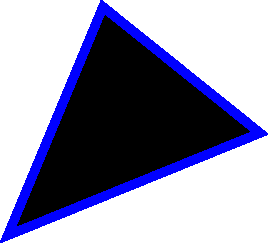
\includegraphics[scale=0.5]{convexhullimages/image_perfect.pdf}
	  \subcaption{Perfect image}
	  \label{fig:image_perfect}
	\end{subfigure}
	\centering
	\begin{subfigure}[b]{0.3\linewidth}
	  \centering
	  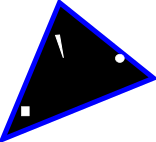
\includegraphics[scale=0.5]{convexhullimages/image_nearperfect.pdf}
	  \subcaption{Near-perfect image}
	  \label{fig:image_nearperfect}
	\end{subfigure}
	\centering
	\begin{subfigure}[b]{0.3\linewidth}
	  \centering
	  
\includegraphics[scale=0.5]{convexhullimages/image_roundedcorners.pdf}
	  \subcaption{Image of rectangle with rounded corners}
	  \label{fig:image_roundedcorners}
	\end{subfigure}
	\centering
	\begin{subfigure}[b]{0.3\linewidth}
	  \centering
	  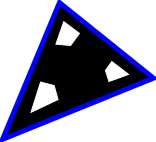
\includegraphics[scale=0.5]{convexhullimages/image_ok.pdf}
	  \subcaption{Ok image}
	  \label{fig:image_ok}
	\end{subfigure}
	\centering
	\begin{subfigure}[b]{0.3\linewidth}
	  \centering
	  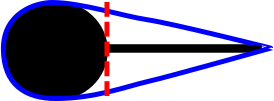
\includegraphics[scale=0.5]{convexhullimages/image_singlesplit.pdf}
	  \subcaption{Image with bad precision which can be fixed by a single split}
	  \label{fig:image_singlesplit}
	\end{subfigure}
	\centering
	\begin{subfigure}[b]{0.3\linewidth}
	  \centering
	  
\includegraphics[scale=0.5]{convexhullimages/image_ring.pdf}
	  \subcaption{Image of a ring with very low precision}
	  \label{fig:image_ring}
	\end{subfigure}
	\centering
	\begin{subfigure}[b]{1.0\linewidth}
	  \centering
	  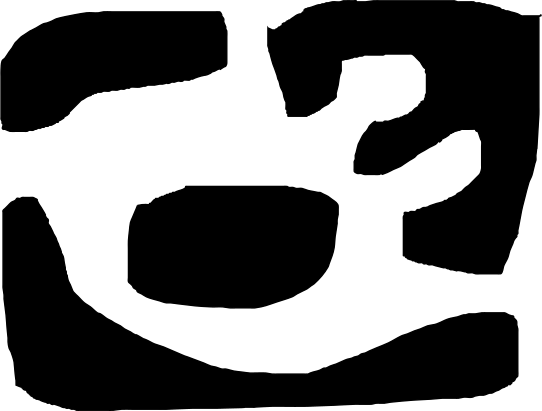
\includegraphics[scale=0.7]{convexhullimages/image_complex.pdf}
	  \subcaption{Large, complex image that has low precision and which is difficult to split manually}
	  \label{fig:image_complex}
	\end{subfigure}
	\centering
	\begin{subfigure}[b]{0.3\linewidth}
	  \centering
	  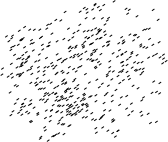
\includegraphics[scale=0.5]{convexhullimages/image_cloud.pdf}
	  \subcaption{Image of a cloud, with very low precision and uniform distribution}
	  \label{fig:image_cloud}
	\end{subfigure}
\caption{Images and convex hulls}
\label{fig:convexhullimages}
\end{figure}

Splitting images can be a difficult and laborious process.
One possible extension to the library would be an automatic splitting algorithm,
that tries to increase the precision with as few different parts as possible.
It should be possible to create such an algorithm that works reasonably well
for many different contexts, but it has not yet been provided in the library.

One possibility is taking the image, finding the longest length, and split the image
in half. Then take the convex hull of each part, and determine how precise each
part is. If the part is not precise enough, the process is repeated recursively for the part.
To avoid recursion, the process stops if the number of parts become too large, or the image
to split becomes too small.
The precision threshold, the number of part to accept (possibly dependent on the image size),
and the size of image to stop at are heuristics that has to be determined somehow
(either manually through testing or automatically through some machine learning and regression
testing).




\subsection{Implementation}

The overall focus of the implementation has been correctness,
safety, robustness and maintainability, as well as asymptotic efficiency.
This focus should help ensure that the library can be extended
improved and changed while still having sufficient efficiency
in most contexts. Constant-factor efficiency has not been prioritized highly.
If improving the library purely for constant-factor efficiency,
try to ensure that the correctness and maintainability is at least
as good as it was before the improvements. Alternatively,
fork the library and modify it to your needs and taste.

The implementation is generally written without side-effects
and with referential transparency. While this does not always
lead to the best constant-factor efficiency,
it helps a lot in regards to maintainability and correctness,
and makes the library easier to use and more predictable.
When modifying the library, try to maintain referential transparency
as far as is appropriate, and document it clearly when referential
transparency is not used.

Exceptions to working with referential transparency
includes tests, performance profiling and demonstrations,
since referential transparency can be somewhat more bothersome
to work with. Examples include randomized tests, GUIs, IO, etc.

In regards to style, it should be noted that if a method or function
that returns a value or object of some sort can fail non-critically,
it should be denoted as such.
In Scala, the return type should thus be Option,
and the method/function name should end in 'O' (as in 'O' for 'Option').
In C++, the return type should be a (possibly managed) pointer,
and the method/function name should end in 'Null'.

As of 2012-05-12, there are no tests, no performance profiling,
and no demonstrations. Improving the library with these parts
would be desirable, but they should be kept outside the core library,
such that users that don't use them doesn't need to use them.

\subsubsection{Scala}

The Scala version is written in an idiomatic, object-functional way.
Modularity is primarily gained through objects,
and correctness and maintainability is gotten through referential
transparency and the advanced type system.

The Scala version uses language version 2.9,
and has no dependencies apart from the core library.

The documentation system is Scaladoc, and SBT is used
for building.

\subsubsection{C++}

The C++ version is not written in a idiomatic way,
mainly because it is a somewhat direct port from Scala.
Scala is generally more expressive than C++ due to its more advanced type system,
its support for garbage collection, and its (collection) libraries
that offers efficient immutable, persistent collections.
Because the C++ version is written in a non-idiomatic way,
it is considerably slower than it could be.
Improving the C++ version to be more idiomatic, more efficient
and still maintainable is highly desirable.

The C++ version is C++11, and uses several features introduced
in C++11. Apart from depending on the standard library, there
are dependencies on Boost.

The documentation system is Doxygen, and CMake is used for building.
There is a implicit dependency on G++, but it should be possible
to change this dependency without too much work, and the library
itself should be fully portable to any system supporting Boost
and C++11.



\section{Appendix}

The appendix describes topics of cursory interest such as
the history of the library.


\subsection{History}

This provides an overview of the development process of the library.

\subsubsection{The beginning and version 0.1}

The library was first motivated by the lack of efficient pixel-perfect collision detection
support, especially in the FOSS community. Many solutions are naive,
simply iterating through all the pixels of one image and testing with the other,
and does not support basic transformations. This is not very flexible or
efficient. Other are slightly more sophisticated,
and supports finding the intersection between axis-aligned bounding boxes.
However, axis-aligned bounding boxes are not a tight fit in a lot of common
cases, and they become even less tight when rotated. In some cases, the implementations
are supported only for languages on certain platforms, such as Flash. Examples include
PMASK (C library) and Collision Detection Kit (ActionScript 3.0 library).
Especially this link was somewhat depressing,
\url{http://stackoverflow.com/questions/5138783/c-2d-pixel-perfect-collision-detection-libraries},
since it clearly seems to implicate that no good pixel-perfect collision detection library exists in C++,
even though C++ is popular for games and computational geometry,
and pixel-perfect collision detection is a library/engine-level
part of games.

The original author of this library decided that the next project
to work on might as well be pixel-perfect collision detection,
and once some basic research into the status of the field was done
(to ensure that no good solution actually existed),
the prototyping was begun. With a background in computer graphics,
algorithms, data structures, game development, mathematics,
linear algebra, image analysis and geometry,
the author had a skill set suitable for completing this challenge.

The basic idea was found fairly early, namely using the intersection
of some polygon to narrow the area to check for as closely as possible.
Since convex hulls are generally very precise or reasonably precise
for a considerable number of applications, and since a convex hull
under scaling/rotation is still a convex hull, it was decided to use convex hulls.
Furthermore, there existed algorithms for finding the intersection
between convex hulls efficiently (namely in linear time).

The earliest prototype was done using Scala and existing libraries.
Scala was used because it can be used with all libraries on the
JVM platform, has high productivity, high safety, high maintainability,
advanced (collection) libraries,
and decent performance compared to C++ and Java.
The library Scalala (Scala Linear Algebra) was used for matrix multiplication,
and the library JTS (JTS Topology Suite) was used for the convex hull intersection.
The Scalala Library was easy to use and performed efficiently,
and was mainly refactored out due to a desire for decreasing dependencies.
The JTS was somewhat easy to use, but didn't perform the convex hull intersection
too efficiently. The reason is likely that JTS is a very general library,
and the convex hull v. convex hull intersection finding was probably supported
by using a more general, but slower algorithm.
Implementing the convex hull intersection algorithm did yield considerable increased performance.

The work with supporting the intersection took considerable time.
However, it was not primarily in the implementation, but in the design phase
that required a lot of time. While the desired algorithm was based upon
an existing algorithm design (see \url{http://www.iro.umontreal.ca/~plante/compGeom/algorithm.html}),
it was an important requirement that the new implementation was geometrically robust.
And that meant handling ALL possible cases correctly.
After a fair bit with experimentation on paper, discovery of cases,
finding general ways to handle issues, etc.,
a possibly correct design was found. As an example of the challenges
of ensuring geometric robustness, in one part of the algorithm about 30 different
cases were identified, which was compressed to about 18 different cases due to
common traits and common handlings.

After some testing and slight debugging (which proved that the overall design
and handling of cases was sane - for instance, one bug was due to the incorrect
identification of a case, and the bugs were fixed by identifying the case correctly),
the prototype was finally done. The testing including textual testing and visual
testing, and some basic performance profiling was also done.

After that, it was decided to port the library to C++.
The reasons include that C++ is close to the metal and
suitable for game library/engine development,
C++ is widely supported by many different vendors and OSs and
C++ is widely used for game library/engine and computational geometry development.
The author had at the beginning not much experience with C++,
nor with porting code from Scala to C++.
Because C++ is a language fraught with dangers and pitfalls,
and the authors experience in C++ was limited,
it was decided to take the 'safe' route and implement
the C++ library in nearly the same way as the Scala library.
While this did give some headaches and trouble,
especially in regards to the type system, the type inference,
the memory handling, the functional programming, templates,
lack of immutable, persistent collections, weird C++-specific behaviours
($vector<bool>$, for instance......for the uninformed,
$vector<bool>$ does not obey the interface for vectors,
due to some weird premature optimization nonsense.
Don't use $vector<bool>$. Use $bitset$, $boost::dynamic\_bitset$ or
$deque<bool>$), it did mean that
once the port was done, the implementation required very little
debugging.

Since the porting was non-idiomatic, it meant that the efficiency
is not nearly as good as it could be, and a simple test
seemed to suggest that the C++ implementation was about 5 times
slower than the Scala implementation for specific cases.
Improving the C++ implementation to become significantly
constant-factor faster should be possible, and it is likely
that making the C++ implementation faster than the Scala
implementation wihtout too much work is likewise possible.

Since the tests was somewhat ad-hoc, it was decided not to
include them in the library.
The library was cleaned up, API-documentation was written,
build systems was used (SBT for Scala, which is very easy,
and CMake for C++), and documentation generation was used
(Scaladoc in SBT for Scala, Doxygen for C++).
These tools generally performed well.

Finally, the manual was written in latex,
images drawn in InkScape,
gitted, and uploaded to github.



\end{document}

